\documentclass[11pt,a4paper,oneside]{article}
\usepackage{color,graphics}
\usepackage{verbatim}
\usepackage{algorithm}
\usepackage{algorithmic}
\usepackage{amsmath}
\usepackage{multirow}
\usepackage{multicol}
%\usepackage{lgrind}
\usepackage[dvips]{graphicx}
\usepackage[T1]{fontenc}
\usepackage{calligra}
\usepackage{xspace}
\usepackage{listings}
\lstset{ 
  language=[GNU]C++,
  frame=tbrl,
  frameround=tttt,
  showspaces=false,
  showtabs=false,
  basicstyle=\footnotesize,
% backgroundcolor=\color{Gray},
% fillcolor=\color{Gray},
  extendedchars=true
}            
\lstloadlanguages{sh,bash,csh,[GNU]C++,[gnu]make,SQL}
\setlength{\oddsidemargin}{0cm}
\setlength{\evensidemargin}{0cm}
\setlength{\topmargin}{-1cm}
\setlength{\textheight}{23cm}
\setlength{\textwidth}{16cm}
\graphicspath{{../ps/}}

\newcommand{\katrin}     {{\sc KATRIN }}
\newcommand{\geant}    {{\sc GEANT4}}
\newcommand{\rootv}    {{\sc ROOT}}
\newcommand{\kemfield}    {{\sc KEMField}}

\newcommand{\squishlist}{
   \begin{list}{$\bullet$}
    { \setlength{\itemsep}{0pt}      \setlength{\parsep}{3pt}
      \setlength{\topsep}{3pt}       \setlength{\partopsep}{0pt}
      \setlength{\leftmargin}{1.5em} \setlength{\labelwidth}{1em}
      \setlength{\labelsep}{0.5em} } }

\newcommand{\squishend}{
    \end{list}  }

\begin{document}

\begin{titlepage}

\begin{figure}
\leftline{ 
\includegraphics[width=0.15\textwidth]{katrin-logo.ps}
\hspace{3.2 cm} 
KATRIN Scientific / Technical Report}
\end{figure} 

\hspace{10.8cm} \today \\ 

\begin{center}

\vspace{1.0cm}

{\Large KEMField - an electrostatic and magnetostatic field solving toolkit \\ } 

\vspace{0.5cm} 

{\large A user's guide for \katrin members\\ }

\vspace{1.0cm}

{\large 
Thomas Corona$^{a}$,
Joseph Formaggio$^{b}$,
Ferenc Gl\"{u}ck$^{c}$, 
}

\vspace{1.0cm}

{\it 
$^{a}$ University of North Carolina at Chapel Hill, USA \\
$^{b}$ Massachusetts Institute of Technology, USA \\ 
$^{c}$ Karlsruhe Institute of Technology, Germany
} 
\vspace{2.0cm} 

\end{center} 

{\large Abstract} \\ 

The electrostatic and magnetostatic field solving software \kemfield, developed and maintained by the \katrin simulation group, is introduced. The document provides a detailed explanation of the installation and implementation of \kemfield, as well as a general description of the structure of the underlying C++ code. 

\end{titlepage}

\tableofcontents
\newpage

\section{Introduction}
\label{sec:intro}

\subsection{Overview}
\label{subsec:overview}

\kemfield\ is a toolkit written in C++ for solving electrostatic and magnetostatic fields from user-defined electrode and magnet configurations.  The Boundary Element Method (BEM) is used to compute discretized charge densities from continuous potential distributions along electrodes \cite{Glueck3},\cite{Poljak}, and the field is computed using a combination of zonal harmonic expansions and direct calculations from geometry primitives using the principle of superposition.  In addition, adaptive-refinement field maps can be generated for commonly accessed regions with computationally complex electric fields.  The techniques employed are adapted from the routines of Dr. Ferenc Gl\"{u}ck \cite{Glueck},\cite{Glueck1},\cite{Glueck2},\cite{Glueck3},\cite{Glueck4},\cite{Glueck5}.  \kemfield\ utilizes the GNU Scientific Library (GSL) \cite{GSL} and ROOT data analysis framework \cite{ROOT} for computation and save/retrieval algorithms, respectively.  \kemfield\ employs both MPI \cite{MPI} and OpenMP \cite{OpenMP} for parallel field computation on a computer grid.  

\subsection{Building the \kemfield\ libraries}
\label{subsec:building}

In order to build the \kemfield\ libraries, the user must first add the main directory (\texttt{KEMField/}) to the \texttt{path} environment variable, and the library directory (\texttt{KEMField/lib}) to the \texttt{LD\_LIBRARY\_PATH} environment variable.  This enables programs to link aginst the \kemfield\ libraries by using the \texttt{KEMField-config} command.  The user must also have GSL (version 1.12 or newer) and ROOT (version 2.24 or newer) installed, with the executables \texttt{gsl\_config} and \texttt{root\_config} correctly identifying the respective library and include paths.  To build the libraries and a suite of test programs, the user need only execute the \texttt{make} command within the top directory\footnote{\kemfield\ has been successfully tested on Mac OS X 10.4, 10.5 and 10.6, as well as several Linux flavors.} \footnote{Thanks to Daniel Furse for his complete revision of the Makefile, making the build process much more dynamic.}.  The included test programs are designed to demonstrate the functionality of different aspects of the \kemfield\ toolkit.  

The libraries can be built to use MPI and OpenMP, if they are installed on the user's operating system.  To use MPI, the user must first set the environment variable \texttt{USE\_MPI}, and then recompile.  Setting this flag causes Both MPI-enabled and MPI-disabled versions of the libraries to be created (the MPI-enabled libraries and executables have the suffix \texttt{\_MPI} in the root of the name).  To use OpenMP, the user must set the environment variable \texttt{USE\_OPENMP} and recompile.  

\subsection{File structure}
\label{subsec:fileStructure}

\subsubsection{Source files}
\label{subsubsec:source}

The source files for \kemfield, located in \texttt{KEMField/Source/}, are divided into folders according to the library to which they belong.  They are:
%
\squishlist
\item \texttt{Geometry}: classes defining the geometry primitives, primitive stores and geometry managers (see Section \ref{sec:geometryPrimitives}),
\item \texttt{BEM}: classes used in performing the matrix algebra associated with the Boundary Element Method of solving for charge densities on electrode sub-elements (see Section \ref{sec:BEM}),
\item \texttt{Direct}: classes used to perform the direct field solving method (see subsection \ref{subsec:direct}),
\item \texttt{ZHExpansion}: classes used to perform the zonal harmonic expansion field solving method (see subsection \ref{subsec:zhHarmonic}),
\item \texttt{FieldMap}: classes used to perform field map generation and field solving using field maps (see subsection \ref{subsec:fieldMap}),
\item \texttt{IO}: classes used to manage the input and output of files and messages for \kemfield,
\item \texttt{Field}: contains the base field solving class (see subsection \ref{subsec:generalProperties}), and the metaclass \texttt{KEMField} (see Section \ref{KEMField}), and
\item \texttt{Test}\footnote{No library is associated with the Test folder.}: main functions for test programs designed to demonstrate the utility of \kemfield.
\squishend
%
Within each folder for which there is an associated library, the source code is divided into header files (\texttt{include/}), source files (\texttt{src/}), and files necessary to link against the ROOT libraries (\texttt{LinkDef/}).  

\subsubsection{Saved files}
\label{subsubsec:saved}

Although the base folder for saved files may be changed by the user, the default configuration is for saved files to be located within \texttt{KEMField/field\_data/saved\_files/}.  Within this folder, ROOT files unique to the electrode and magnet geometry are read and written, and the folder \texttt{fieldmap/} contains data pertinent to a generated field map (if one exists).  The folder \texttt{field\_data/} also contains the folder \texttt{images/} for storing test images generated by certain test programs, and \texttt{input\_files/}, where geometry cards are kept (see subsection \ref{subsubsec:cardReaders}).  

\subsubsection{Other files}
\label{subsubsec:other}

In keeping with commonly accepted UNIX programming standards, generated executables designed to test, validate and demonstrate the utility of \kemfield\ are located in \texttt{KEMField/bin/}, generated libraries are located in \texttt{KEMField/lib/}, temporary files are stored in \texttt{KEMField/tmp/}, and scripts associated to \kemfield\ (document generating scripts and submission scripts for various grids) are kept in \texttt{KEMField/scripts/}.  The documentation for \kemfield\ (including the document you are reading) is located in \texttt{KEMField/doc/}.  Finally, the executable shell script \texttt{KEMField-config} is designed for use by other programs to link against the libraries of \kemfield, in keeping with the standard \texttt{*-config} format.  

\section{Class \texttt{KEMField}: the user interface}
\label{KEMField}

In addition to being the name of the toolkit described by this document, \texttt{KEMField} is also the name of the top-level class through which the user accesses the geometry and field solving classes (to avoid ambiguity, \texttt{KEMField}, in this font, will hereafter always refer to the class, and \kemfield\ to the toolkit).  

\subsection{Adding field solvers}
\label{subsec:addingFieldSolvers}

When an instance of \texttt{KEMField} is created, it has associated with it an electrode and magnet manager (see subsection \ref{subsec:managingPrimitives}), but by default there are no field solving methods.  The user must choose which methods are appropriate to the simulation being performed, and in what order they should be used.  An example of adding field solvers to an instance of \texttt{KEMField} is demonstrated below:
%
\begin{lstlisting}[language=C++]
  ...
  // construct an instance of KEMField
  KEMField* field = new KEMField();
  
  // a general verbosity setting for managers and field solvers
  Int_t verbose = 3;
  
  // access the electrode and magnet managers
  KElectrodeManager* eManager = field->GetElectrodeManager();
  KMagnetManager*    mManager = field->GetMagnetManager();
  
  // add a direct electric field solver to KEMField
  field->AddEFieldSolver(new KEDirectFieldSolver(eManager));

  if (eManager->CheckForAxialSymmetry())
  {
    // if the simulation is axially symmetric, add a zonal harmonic electric
    // field solver to KEMField
    field->AddEFieldSolver(new KEZHFieldSolver(eManager));

    // set the solver to the highest priority (NB: the field solver can be
    // accessed by name or by its index within KEMField)
    field->SetPriority("KEZHFieldSolver",1);
    
    // set the field solver's verbosity level
    field->SetVerbose("KEZHFieldSolver",verbose);
  }
    
  // set the direct field solver's priority level to be lower than that of
  // the zonal harmonic electric field solver
  field->SetPriority("KEDirectFieldSolver",3);
  
  // set the field solver's verbosity level
  field->SetVerbose("KEDirectFieldSolver",verbose);

  // add a direct magnetic field solver to KEMField
  field->AddBFieldSolver(new KMDirectFieldSolver(mManager));
  
  // add a zonal harmonic magnetic field solver to KEMField
  field->AddBFieldSolver(new KMZHFieldSolver(mManager));
  
  // set the magnetic field solver's priorities
  field->SetPriority("KMZHFieldSolver",1);
  field->SetPriority("KMDirectFieldSolver",2);

  // set the field solvers' verbosity levels
  field->SetVerbose("KMZHFieldSolver",verbose);
  field->SetVerbose("KMDirectFieldSolver",verbose);
  
  // set the electrode and magnet manager's verbosity levels
  // (this could also have been done by accessing the managers directly)
  field->SetVerbose("KElectrodeManager",verbose);
  field->SetVerbose("KMagnetManager",verbose);
    ...
\end{lstlisting}
%
Once a field solver is added to an instance of \texttt{KEMField}, \texttt{KEMField} takes ownership of it.  In other words, when the user deletes the instance of \texttt{KEMField} that was created above, all of the field solvers (and, naturally, the geometry managers) are deleted with it.  While more than one instance of \texttt{KEMField} can exist at once, the user must take care when sharing field solvers between distinct instances of \texttt{KEMField}.  

\subsection{Initializing the geometry managers and field solvers}
\label{subsec:initializing}

Since the geometry managers both share the same underlying structure, and the field solving classes conform to a base model, it is possible to initialize the instance of \texttt{KEMField} for use in field solving by merely executing the command 
%
\begin{lstlisting}[language=C++]
  ...
  field->Initialize();
  ...
\end{lstlisting}
%
The preparation of the geometry and field solvers is then taken care of by \texttt{KEMField}, and no other user input is necessary.  Once the geometry is loaded into the managers and the \texttt{KEMField} instance is initialized, the user is ready to compute electric and magnetic fields and potentials.  

\subsection{Accessing the electric and magnetic field and potential}
\label{subsec:accessing}

In order to get field and potential values from \texttt{KEMField}, the following functions are used:
%
\squishlist
\item \texttt{void CalculateBField(const Double\_t P[3], Double\_t field[6]) const}: computes the magnetic field at $\texttt{(P[0],P[1],P[2])}$.  The first 3 components of \texttt{field[6]} correspond to the x, y, and z-components of the magnetic field, and the last 3 the electric field (GEANT format).  
\item \texttt{void CalculateEField(const Double\_t P[3], Double\_t field[6]) const}: computes the electric field at $\texttt{(P[0],P[1],P[2])}$.
\item \texttt{void CalculateField(const Double\_t P[3], Double\_t field[6]) const}: computes both the electric and magnetic fields at $\texttt{(P[0],P[1],P[2])}$.
\item \texttt{void CalculateBPotential(const Double\_t P[3], Double\_t field[6]) const}: computes the magnetic vector potential at $\texttt{(P[0],P[1],P[2])}$.  The first component of \texttt{phi[4]} corresponds to the electric potential, and the last 3 the magnetic vector potential $\vec{A} = (A_{x},A_{y},A_{z})$.  
\item \texttt{void CalculateEPotential(const Double\_t P[3], Double\_t field[6]) const}: computes the electric potential at $\texttt{(P[0],P[1],P[2])}$.  
\item \texttt{void CalculatePotential(const Double\_t P[3], Double\_t field[6]) const}: computes both the electric potential and the magnetic vector potential at $\texttt{(P[0],P[1],P[2])}$.  
\squishend
%
A complete demonstration of their use is given in the test program \texttt{bin/TestEMField}.  

\section{Geometry primitives}
\label{sec:geometryPrimitives}

\subsection{Available primitives}
\label{subsec:availablePrimitives}

\begin{table}
\centering
\begin{tabular}{|c|c||c|c|}
\hline
Geometry & Graphical & Geometry & Graphical\\
Primitive & Description & Primitive & Description\\
\hline
& \multirow{3}{*}{\includegraphics[scale=.18]{wire.ps}} & &
\multirow{3}{*}{\includegraphics[scale=.18]{conicSect.ps}} \\
\texttt{KTWireElectrode} & & \texttt{KTConicSectElectrode} & \\
\it{(collective)}& & \it{(singular)} & \\
& & & \\
\hline
& \multirow{3}{*}{\includegraphics[scale=.18]{triangle.ps}} & &
\multirow{3}{*}{\includegraphics[scale=.18]{loop.ps}} \\ 
\texttt{KTTriangleElectrode} & & \texttt{KTRingMagnet} & \\
\it{(collective)}& & \it{(singular)} & \\
& & & \\
\hline
& \multirow{3}{*}{\includegraphics[scale=.18]{ring.ps}} & &
\multirow{3}{*}{\includegraphics[scale=.18]{solenoid.ps}} \\
\texttt{KTRingElectrode} & & \texttt{KTSolenoidMagnet} & \\
\it{(singular)}& & \it{(singular)} & \\
& & & \\
\hline
& \multirow{3}{*}{\includegraphics[scale=.18]{rectangle.ps}} & &
\multirow{3}{*}{\includegraphics[scale=.18]{coil.ps}} \\
\texttt{KTRectangleElectrode} & & \texttt{KTCoilMagnet} & \\
\it{(collective)}& & \it{(singular)} & \\
& & & \\
\hline
\end{tabular}
\caption{Available electrode and magnet geometry primitives.  Collective primitives can be represented as repeated instances about the azimuthal axis, demonstrating discrete rotational symmetry.  Singular primitives inherently have continuous rotational symmetry, and are therefore represented  as singular instances.}
\label{primitiveTable}
\end{table}
%
Electrodes can be arranged in a general 3-dimensional configuration using wires, rectangles and triangles, but axially symmetric (or approximately axially symmetric) electrode configurations consisting of conic sections and repeated wires, rectangles and triangles about the azimuthal axis are preferable, as they facilitate the use of faster field computation algorithms.  Currently supported magnets include wire loops, solenoids and thick coils (electromagnets), each of which can be defined according to its own symmetry axis.  A graphical description of the available electrode and magnet primitives can be seen in Table \ref{primitiveTable}.

Depending on their symmetry properties, electrode primitives are either represented as singular instances or as collections of identical sub-elements repeated about the azimuthal axis.  For example, a \texttt{KTConicSectElectrode} describes a single conic section electrode with only one placement in the system because it is naturally axially symmetric, whereas a \texttt{KTWireElectrode} can describe a collection of multiply placed wire segments about the azimuthal axis.  In addition, each electrode type can be placed into a \texttt{KTElectrodeGroup}, where the group of electrodes is treated as a single independent electrode primitive during the implementation of the BEM.  

Currently, only magnet primitives that have rotational symmetry about one of its axes are represented in \kemfield .  There are therefore no collective magnet primitives, as all supported magnets are singular primitives.  Since the computation of the magnetic field from a magnet description is more straightforward than for its electric counterparts, and because magnet discretization and implementation of the BEM are unnecessary, there is no need to group magnets for the simplification of a BEM calculation.  Instead, magnets are grouped that share a common axis of symmetry, allowing for multiple magnet groups that have different symmetry axes.  The grouping of coaxial magnets is done in much the same way that electrodes are grouped, using instances of \texttt{KTMagnetGroup}.  Examples of electrode and magnet groups can be seen in the program \texttt{bin/TestGeometry}.

\subsection{Adding primitives to the simulation}
\label{subsec:addingPrimitives}

\subsubsection{Manually adding primitives}
\label{subsubsec:manuallyAddingPrimitives}

An example of manually creating geometry primitives and adding them to the simulation is displayed below:
%
\begin{lstlisting}[language=C++]
#include <cstdlib>
#include <iostream>

#include "KElectrodeManager.hh"

#include "KTConicSectElectrode.hh"
#include "KTWireElectrode.hh"

int main(Int_t argc, char* argv[])
{
  // Construct a single conic section electrode.
  KTConicSectElectrode* c = new KTConicSectElectrode(0,       // z_A (m)
						     .5,      // r_A (m)
						     1,       // z_B (m)
						     .5,      // r_B (m)
						     1,       // potential (V)
						     5);      // numDisc

  // Construct fifty wires with discrete rotational symmetry about the
  // azimuthal axis.
  Double_t a[3] = {1,1,1}; // x,y,z of 1st endpoint of 1st copy (m)
  Double_t b[3] = {3,1,2}; // x,y,z of 2nd endpoint of 1st copy (m)
  
  KTWireElectrode* w = new KTWireElectrode(a,
					   b,
					   .05,// diameter of the wire (m)
					   10, // potential of the wire (V)
					   50, // # of wires about the azi. axis
					   10);// numDisc

  // Construct a new electrode manager.
  KElectrodeManager* eManager = new KElectrodeManager();

  // Add the conic section electrode to the manager.
  eManager->Add(c);

  // Add the wire electrodes to the manager.
  eManager->Add(w);

  // When a primitive is added to the manager, a copy of the primitive is
  // constructed as an object within the manager's storage classes.  The
  // original primitive is no longer needed, and can be deleted by the user.
  delete c;
  delete w;
  ...
\end{lstlisting}
%
Note that, when an electrode is added to the simulation, a copy of its parameters is passed to the appropriate storage classes.  This means that the same electrode can be modified and added to the simulation multiple times, reducing the number of times the user must call \texttt{new} and \texttt{delete}.  

\subsubsection{Card readers}
\label{subsubsec:cardReaders}

Alternatively, geometry primitives can be loaded into a simulation via \texttt{Elcd3\_2}, \texttt{Elcd3\_3}, and \texttt{Magfield3}-style cards.  Card readers exist for conic section, rectangle, triangle and wire electrodes, and for coil magnets.  Cards that are read into the simulation can be commented by using the escape character "\#".  Card readers can be used independently (see test program \texttt{bin/TestCardInput}), or in conjunction with \texttt{KEMField} with the function
%
\begin{lstlisting}[language=C++]
    void KEMField::ReadGeometryFromCards(std::string ConicSectFileName,
                                         std::string CoilFileName,
                                         std::string RectangleFileName,
                                         std::string WireFile,
                                         std::string TriangleFileName);
\end{lstlisting}

%\subsubsubsection{Example Cards}
%\label{subsubsubsec:exampleCards}
\paragraph{Example Cards:} The following are sample cards for conic sections, rectangles, wires and magnets.  
%
\begin{lstlisting}[language=sh]
# inputfull.dat

# total number of conic sections described by the file

2

# the following 6 parameters are described as follows:
#     1: z-coordinate of the 1st endpoint of the generating line (m)
#     2: r-coordinate of the 1st endpoint of the generating line (m)
#     3: z-coordinate of the 2nd endpoint of the generating line (m)
#     4: r-coordinate of the 2nd endpoint of the generating line (m)
#     5: Potential at which the electrode is held (V)
#     6: the number of conic sections into which the conic section
#        will be discretized (0 if no discretization)

1.5	1	3	1	50	10

# the next 6 parameters are identical in meaning to the previous line,
# for the second conic section

3   0	3	1	0	5
\end{lstlisting}
%
\begin{lstlisting}[language=sh]
# inputrectangle.dat

# total number of rectangles described by this file

2

# the following 16 parameters are described as follows:
# 1: The index is the number of the rectangle in the file. It starts
#    at 1 for the first rectangle, and increments by one for each
#    subsequent rectangle.
# 2: This parameter indicates to which KTElectrodeGroup the rectangle
#    belongs. Rectangles that are in the same group must be placed
#    together in the file, and the group parameter must start at one and
#    increment by only one (for rectangles within the same group, it does
#    not increment at all). Alternatively, the group parameter can be set
#    to -1 for all of the rectangles, indicating that the rectangles are
#    not grouped.
# 3: This parameter is not used by the card reader.
# 4: For repeated rectangles about the azimuthal axis, this parameter
#    sets the number of repeated instances of the rectangle the program
#    should create. The # of replicas must be greater than or equal to
#    one; if a rectangle is not repeated about the azimuthal axis, the
#    parameter should be set to one.
# 5,6,7: The x, y, and z-coordinates of a corner of the rectangle (m)
# 8,9,10: the unit vector pointing from P0 along the longer side of
#         the rectangle (side A)
# 11,12,13: the unit vector pointing from P0 along the shorter side of
#           the rectangle (side B)
# 14: the magnitude of the longer side (A) of the rectangle (m)
# 15: the magnitude of the shorter side (B) of the rectangle (m)
# 16: the potential of the electrode (V)

1  1  0  10  0  10.  0  1  0  0  0  1  0  .05  .05  10

# the next 16 parameters are identical in meaning to the previous
# line, for the second rectangle

2  2  0  1  0  0  1  1  0  0  0  1  0  1  1  1
\end{lstlisting}
%
\begin{lstlisting}[language=sh]
# inputwire.dat

# total number of wires described by this file

1

# the following 16 parameters are described as follows:
# 1: The index is the number of the wire in the file. It starts at 1
#    for the first wire, and increments by one for each subsequent
#    wire.
# 2: This parameter indicates to which KTElectrodeGroup the wire
#    belongs. Wires that are in the same group must be placed together in
#    the file, and the group parameter must start at one and increment by
#    only one (for wires within the same group, it does not increment at
#    all). Alternatively, the group parameter can be set to -1 for all of
#    the wires, indicating that the wires are not grouped.
# 3: This parameter is not used by the card reader.
# 4: For repeated wires about the azimuthal axis, this parameter sets
#    the number of repeated instances of the wire the program should
#    create. The # of replicas must be greater than or equal to one; if a
#    wire is not repeated about the azimuthal axis, the parameter should
#    be set to one.
# 5,6,7: These three parameters describe the x, y, and z-coordinates
#        of one end of the wire (m).
# 8,9,10: These three parameters describe the x, y, and z-coordinates of
#         the other end of the wire (m).
# 11: Describes the diameter of the wire (m).
# 12,13,14,15: These parameters are not used by the card reader.
# 16: Describes the potential of the electrode (V).

1 -1 0 10 .5 .5 -.15 .5 .5 .15 .05 0 0 0 0 100
\end{lstlisting}
%
\begin{lstlisting}[language=sh]
# inputcoil.dat

# total number of magnets described by the file

2

# the following 13 parameters are described as follows: 
#     1,2,3:	global (x,y,z) of local origin
#     4,5,6:	global (x,y,z) of local (1,0,0)
#     7,8,9:	global (x,y,z) of local (0,1,0)
#     10,11,12:	global (x,y,z) of local (0,0,1)
#     13:	number of magnets defined within this cooridnate frame
#
# numbers may be separated by tabs or spaces (or both)

0   0   0   1.   0   0   0   1.   0   0   0   1.   2

# the following 5 parameters are described as follows:
#     1: the z-coordinate of the middle of the magnet (m)
#     2: the minimum r-coordinate of the magnet  (m)
#     3: the thickness of the magnet in the r-direction  (m)
#     4: the length of the magnet in the z-direction  (m)
#     5: the total current in the magnet (A)

-2.15    0.227  0.043   0.320   2120000.

# the next 5 parameters are identical in meaning to the previous line,
# for the second magnet defined within this coordinate frame

2.15     0.227  0.043   0.320   2120000.
\end{lstlisting}


\subsubsection{KXML, other interfaces}
\label{subsubsec:otherInterfaces}

Alternative methods for adding geometry primitives to \kemfield, including {\sc KXML}\cite{Furse} and direct inputs from the \katrin database, are currently being developed.  

\subsection{Managing geometry primitives}
\label{subsec:managingPrimitives}

The interfaces between electrode and magnet primitives created by the user and the field solving routines employed in \kemfield\ are \texttt{KElectrodeManager} and \texttt{KMagnetManager}, respectively.  By interacting with the electrode and magnet managers, the user is able to:
%
\squishlist
\item Add and retrieve electrodes/magnets
\item Set the reflectional symmetry of the simulation (electrodes only)
\item Discretize electrodes (used for constant charge density approximation)
\item Save and retrieve electrode/magnet geometries from file
\squishend
%
The electrode and magnet managers contain methods that automate the preparation of a geometry configuration for use in field computation.  Once the geometry primitives have been loaded into their respective managers, the user need only execute the commands 
%
\begin{lstlisting}[language=C++]
  ...
  eManager->Initialize();
  mManager->Initialize();
  ...
\end{lstlisting}
%
and the requisite steps are taken to enable field computation\footnote{When used within the context of the class \texttt{KEMField}, the managers are automatically initialized as part of \texttt{KEMField::Initialize()}.}.  Feedback from the manager classes can be printed to the screen by setting the verbosity of each class (\texttt{e/mManager->SetVerbose(\#)}) from 0 (silent) to 5 (most verbose).  The general steps of the initialization methods are outlined below.  

\subsubsection{Save and retrieval of geometry configurations}
\label{subsubsec:saveRetrieve}

When a geometry configuration is inputted into the simulation, a check is performed to determine whether or not a similar configuration has been processed during a prior simulation.  The default locations and names for file saving/retrieving is \texttt{KEMField/field\_data/saved\_files/electrodes.root} and \texttt{KEMField/field\_data/saved\_files/magnets.root}, but can be changed prior to initialization by executing the commands
%
\begin{lstlisting}[language=C++]
  ...
  eManager->SetSaveFileName(filename);
  eManager->SetRetrieveFileName(filename);

  mManager->SetSaveFileName(filename);
  mManager->SetRetrieveFileName(filename);
  ...
\end{lstlisting}
%
The manager classes determine if the loaded configuration is
%
\squishlist
\item identical to a previous simulation, 
\item geometrically equivalent to a previous simulation, but with electrodes held at different potential values, 
\item geometrically similar to a previous simulation, with identical potential values, or 
\item completely different from all previous simulations.
\squishend
%
Each of these situations is handled differently during the computation of charge densities, which is explained in Section \ref{sec:BEM}.  When a new file is to be created, its name is the chosen (or default) save name root, appended with \texttt{\_\#.root} when a file with that name already exists.  During the comparsion against preexisting files, all files with the same name root are compared against the current geometry.  

\subsubsection{Electrode discretization}
\label{subsubsec:electrodeDiscretization}

One of the approximations of the BEM is the assumption of constant charge density across an electrode.  It is therefore necessary to discretize the electrode primitives added to the simulation into smaller sub-elements, so the approximation can be held valid.  Each electrode primitive in \kemfield\ has a method associated with it that automates this process, discretizing itself into smaller electrodes according to an associated discretization parameter (passed to the electrode in its constructor), as well as a static parameter associated with each primitive type.  The discretization of electrodes is performed once all of the electrodes are added into the simulation.  

\subsubsection{Computation of electrode charge densities}
\label{subsubsec:computationOfChargeDensities}

The computation of electrode charge densities is performed using the BEM.  A more detailed explanation of this procedure is given in Section \ref{sec:BEM}.

\subsubsection{Axially symmetric and asymmetric approximations}
\label{subsubsec:symApproximations}

Once the electrodes are discretized and the charge densities for each electrode have been computed, symmetry-related approximations can be made.  For electrode configurations that are nearly axially symmetric, primitives with discrete rotational symmetry can be approximated as axially symmetric electrodes.  The approximated electrode will be used in lieu of the original electrode when the field point to be computed is sufficiently far from the electrode (scalable by a user-defined parameter).  Each collective electrode class contains a method for performing this approximation.  

Additionaly, electrode configurations that contain axially symmetric electrodes but in general are {\it not} axially symmetric must be converted into a completely asymmetric configuration, in order to allow for a varying charge density about the aximuthal axis.  Each singular electrode class contains a method for performing this approximation.  

\section{The Boundary Element Method}
\label{sec:BEM}

\subsection{Overview}
\label{subsec:BEMOverview}

The theory behind the computation of the charge densities on electrode sub-elements via the BEM is explained in \cite{Glueck5}, \cite{Corona}.  Procedurally, the task of the BEM classes is to solve the linear algebraic equation
%
\begin{equation}
U_{i} = W_{ij} \cdot \sigma_{j}
\label{eq:BEMLinAlg}
\end{equation}
%
for $\sigma_{j}$, where $U_{i}$ is the electric potential of electrode $i$, $W_{ij}$ is the geometric component of the electric potential at a point centered on electrode $i$ due to electrode $j$, and $\sigma_{j}$ is the charge density on electrode $j$.  \kemfield\ employs three methods for solving this equation:
%
\squishlist
\item Gaussian elimination, 
\item inversion of the matrix $W_{ij}$, and
\item Gauss-Seidel method of successive displacement.  
\squishend
%
The BEM is employed automatically during the initialization method of the electrode manager.  

\subsection{Gaussian elimination and matrix inversion}
\label{subsec:gaussianElimMatrixInvert}

For electrode configurations that are entirely dissimliar to those of previously computed simulations, one of the first two methods (selected by a user-defined parameter) is employed to solve for the components of the $\sigma_{j}$ vector.  While Gaussian elimination is faster than complete matrix inversion, the latter method has the benefit of facilitating the speed of future computations, where a geometry configuration differs from the current one only by differences in the potential values on the electrodes.  When it is used, the method of matrix inversion saves the computed inverted matrix to file.  Future simulations that vary in potential only can then be rapidly solved by simply multiplying this matrix with the new potential values.  Both methods are written for serial computation and for MPI-enabled parallel computation using techniques from \cite{Karniadakis} for use in distributed computing.  

\subsection{Gauss-Seidel method of successive displacement}
\label{subsec:gaussSeidel}

The third method is used when a previously computed simulation differs geometrically only slightly from the current configuration, and the initial approximate values for the charge densities can be taken from the previous simulation.  When the conditions for its use are appropriate, the Gauss-Seidel method is the fastest method for solving the linear algebraic equation.  However, the method is not readily transferrable into parallel computation, and must be performed serially.  

\section{Field Solvers}
\label{sec:fieldSolvers}

\subsection{General Properties}
\label{subsec:generalProperties}

Once the geometry is prepared (electrodes and magnets inputted into their respective managers, electrodes discretized and charge densities computed, symmetry approximations made, and files saved), the user then selects the field solvers to be used in the simulation.  All field solvers inherit from the parent class \texttt{KEMFieldSolver}, and can perform the following basic tasks: 
%
\squishlist
\item \texttt{std::string GetName()}: returns the name of the field solver.
\item \texttt{void Initialize()}: prepares the field solver for use in simulation.  
\item \texttt{Bool\_t FieldCanBeComputedAtPoint(const Double\_t P[3])}: returns true if the field solver is valid at $\texttt{(P[0],P[1],P[2])}$, false if it is not.  
\item \texttt{void CalculateField(const Double\_t P[3], Double\_t field[6])}: computes the field at $\texttt{(P[0],P[1],P[2])}$.  The first 3 components of \texttt{field[6]} correspond to the x, y, and z-components of the magnetic field, and the last 3 the electric field (GEANT format).  
\item \texttt{void CalculatePotential(const Double\_t P[3], Double\_t phi[4])}: computes the electric potential and magnetic vector potential at $\texttt{(P[0],P[1],P[2])}$.  The first component of \texttt{phi[4]} corresponds to the electric potential, and the last 3 the magnetic vector potential $\vec{A} = (A_{x},A_{y},A_{z})$.  
\item \texttt{void SetVerbose(Int\_t i)}: like the manager classes, sets the verbosity of the solver.  
\item \texttt{void SetPriority(Int\_t i)}: Sets the priority of the solver.  This is explained in more detail in Section \ref{KEMField}.  
\squishend
%

\subsection{Direct calculation method}
\label{subsec:direct}

\begin{lstlisting}[language=C++]
  ...
  KEDirectFieldSolver* dESolver = new KEDirectFieldSolver(eManager);
  KMDirectFieldSolver* dMSolver = new KMDirectFieldSolver(mManager);
  ...
\end{lstlisting}

Direct field solvers (\texttt{KEDirectFieldSolver}, \texttt{KMDirectFieldSolver}) are so named because they compute the electric potential, magnetic vector potential, and electric and magnetic fields using techniques based on analytic forms specific to each geometry primitive.  Derivations of the formulae used to perform these calculations can be found in \cite{Glueck3}, \cite{Glueck4}, \cite{Glueck5}, \cite{Corona}.  

When possible, analytic techniques for determining the electric field from a geometry primitive are used.  If an analytic form has not been derived, the electric field is computed using numeric differentiation of the electric potential.  Using the law of superposition, the field values are computed as merely the sum of the contributions from each sub-element.  If OpenMP is enabled, these sums are performed in parallel.  

\subsection{Zonal harmonic expansion method}
\label{subsec:zhHarmonic}

Geometry configurations that are axially symmetric (or approximately axially symmetric) can be solved using the method of zonal harmonic expansion by envoking the classes \texttt{KEZHFieldSolver} and \texttt{KMZHFieldSolver}.  The method solves for the electric and magnetic field and potential by computing series similar to the following forms:
%
\begin{equation}
\Phi_{cen}(r_{cyl},z_{cyl}) = \sum_{n=0}^{\infty} \Phi^{cen}_{n}|_{z_{0}} \left( \frac{\rho}{\rho_{cen}}\right)^{n} P_{n}(\cos{\theta}),
\label{phiLegendreCen}
\end{equation}
%
\begin{equation}
\Phi_{rem}(r_{cyl},z_{cyl}) = \sum_{n=0}^{\infty} \Phi^{rem}_{n}|_{z_{0}} \left( \frac{\rho}{\rho_{rem}}\right)^{-(n+1)} P_{n}(\cos{\theta}),
\label{phiLegendreRem}
\end{equation}
%
for multiple $z_{0}$ source points along the axis of rotational symmetry.  This method is explained in detail in \cite{Glueck1}, \cite{Glueck2}, \cite{Corona}.  

Prior to initialization, parameters that characterize the zonal harmonic expansion technique can be set as follows:

\begin{lstlisting}[language=C++]
  ...
  KEZHFieldSolver* zhEFieldSolver = new KEZHFieldSolver(eManager);
  zhEFieldSolver->SetZHParameters((Double_t) prox_to_sp,
                                  (Double_t) convergenceParam,
                                  (Double_t) spSpacing,
                                  (Double_t) convergenceRatio,
                                  (Int_t)    nCenCoeffs,
                                  (Int_t)    nRemCoeffs,
                                  (Int_t)    nBifurcations);

  KMZHFieldSolver* zhMFieldSolver = new KMZHFieldSolver(eManager);
  zhMFieldSolver->SetZHParameters((Double_t) prox_to_sp,
                                  (Double_t) convergenceParam,
                                  (Double_t) spSpacing,
                                  (Double_t) convergenceRatio,
                                  (Int_t)    nCenCoeffs,
                                  (Int_t)    nRemCoeffs,
                                  (Int_t)    nBifurcations);
  ...
\end{lstlisting}
%
where the paramaters are defined as:
%
\squishlist
\item \texttt{Double\_t prox\_to\_sp}: if the distance between a field point and a source point is less than this tolerance, only the first terms of the series are used,
\item \texttt{Double\_t convergenceParam}:  when the last term in the series is smaller than the former term by this parameter, the summation ends,
\item \texttt{Double\_t spSpacing}: the distance along the z-axis between source points,
\item \texttt{Double\_t convergenceRatio}: when $\frac{\rho}{\rho_{cen}}$ or $\frac{\rho_{rem}}{\rho}$ is less than this ratio, the expansion method is valid for use,
\item \texttt{Int\_t nCenCoeffs}: the maximum number of terms used in each central expansion,
\item \texttt{Int\_t nRemCoeffs}: the maximum number of terms used in each remote expansion, and
\item \texttt{Int\_t nBifurcations}: the maximum number of subdivided geometry collections.  This is explained in further detail in \ref{subsubsec:collections}.
\squishend

\subsubsection{Collections}
\label{subsubsec:collections}

Both electric and magnetic geometry primitives are grouped into \emph{collections} in order to extend the utility of the method of zonal harmonic expansion.  Geometry primtives are gouped according to spacial proximity, allowing for a partial zonal harmonic calculation of fields even if the field point is close to one of the collections of primitives.  The grouping of electrodes is performed by repeatedly bifurcating the electrode geometry along the z-axis (the number of bifurcations is set by the user).  For magnetic geometry primitives, collections are used to group magnets with a common axis of symmetry, and these groups are subdivided [\texttt{nBifurcations}] times.  If OpenMP is enabled, the series expansions for different collections are performed in parallel.  

\subsection{Interpolation from field maps}
\label{subsec:fieldMap}

For regions in which the computation of electric fields is computationally expensive, adaptive-refinement field maps spanning the region can be constructed beforehand.  Once the field maps are generated, a fourth order reduced multivariate Hermite interpolator is used to compute the electric potential and electric field to a user-defined tolerance.  The technique is discussed in more detail in \cite{Corona}.  

\subsubsection{Constructing field maps}
\label{subsubsec:constructingFieldMaps}

Field maps may be constructed in serial for both axially symmetric and asymmetric electrode configurations as follows: 

\begin{lstlisting}[language=C++]
  ...
  // construct an instance of KEMField
  KEMField* field = new KEMField();

  ...
  // add field solvers to the instance of KEMField
  ...

  // create a pointer to a general (2-dimensional or 3-dimensional) field map
  KFieldMap_base* fm;

  Double_t tolerance   = 1.e-3; // tolerance across the field map
  Double_t maxCubeSize = 1.; // size of a side of the largest cube (m)
  Int_t  nLevel    = 3; // # of times the largest cube can be subdivided

  // ...to make the tolerance better reflect the accuracy...
  tolerance*=.1;

  if (eManager->CheckForAxialSymmetry())
  {
    // construct a 2-dimensional field map for the axially symmetric field
    fm = new KFieldMap_2D(field,tolerance,maxCubeSize,nLevel);
    // Set the (r_min, r_max, z_min, z_max) dimensions of the map (in meters)
    fm->SetDimensions(0,3,1.5,5.5);
  }
  else
  {
    // construct a 3-dimensional field map for the asymmetric field
    fm = new KFieldMap_3D(field,tolerance,maxCubeSize,nLevel);
    // set the (x_min,x_max,y_min,y_max,z_min,z_max) dimensions
    // of the map (in meters)
    fm->SetDimensions(-3,3,-3,3,-3,3);
  }
    
  // construct the primary grid, save the header information
  fm->InitializeFieldMap();

  for (Int_t i=0;i<fm->GetNMetaCubes();i++)
  {
    // fill each cube in the primary grid
    fm->FillMetaCube(i);
  }
    ...
\end{lstlisting}
%
The user-defined parameters that characterize a field map are:
%
\squishlist
\item \texttt{Double\_t tolerance}: the average error of the interpolated value computed from the field map
\item \texttt{Double\_t maxCubeSize}:  the length of a side of the top-level cube.  The initial map is formed by dividing the region into cubes with this side length, and subsequent cubes are formed by subdividing these cubes.  Top-level cubes that contain an electrode are removed from the map, as a uniform tolerance cannot be guaranteed in this region.  
\item \texttt{Int\_t nLevel}: the maximum number of times a top-level cube is subdivided in order to attain the appropriate tolerance.
\item \texttt{Double\_t dimensions[4 or 6]}: the 2- (or 3-) dimensional coordinates of the field map.
\squishend

While the methods for computing a field map in serial produce the same results as their parallel counterpart, the preferred method for field map construction is in parallel on an MPI-enabled computer grid.  An example program that performs exactly this task, \texttt{bin/TestFieldMap\_MPI}, and its source are provided for the user.  

\subsubsection{Implementing field maps for use in computation}
\label{subsubsec:constructingFieldMaps}

As they inherit from \texttt{KEMFieldSolver}, the classes \texttt{KFieldMap\_2D} and \texttt{KFieldMap\_3D} are implemented in much the same way as the other field solvers.  However, since a field map used for computing fields must already be generated, the user-defined parameters that characterize the map are taken from the saved configuration of the map itself, rather than set by the user.  An example of their implementation is given below:
%
\begin{lstlisting}[language=C++]
  ...  
  // create a pointer to a general (2-dimensional or 3-dimensional) field map
  KFieldMap_base* fm;

  if (eManager->IsAxiallySymmetric())
    fmEFieldSolver = new KFieldMap_2D((KEMPrimitiveManager*)eManager);
  else
    fmEFieldSolver = new KFieldMap_3D((KEMPrimitiveManager*)eManager);
  ...
\end{lstlisting}

\begin{thebibliography}{99}

	\bibitem{Glueck3}
	  Ferenc Gl\"{u}ck,
	  \emph{Axisymmetric electric field calculation by BEM and elliptic integrals}.
	  to be published.

	\bibitem{Poljak}
	  D. Poljak and C. A. Brebbia,
	  \emph{Boundary Element Methods for Electrical Engineers}.
	  WIT Press, Boston,
	  1st Edition,
	  2005.

	\bibitem{Glueck}
	  Ferenc Gl\"{u}ck,
	  \emph{Untitled- research notes and personal correspondence}.

	\bibitem{Glueck1}
	  Ferenc Gl\"{u}ck,
	  \emph{Axisymmetric electric field calculation by zonal harmonic expansion}.
	  to be published.

	\bibitem{Glueck2}
	  Ferenc Gl\"{u}ck,
	  \emph{Magnetic field calculation of coils by zonal harmonic expansion}.
	  to be published.

	\bibitem{Glueck4}
	  Ferenc Gl\"{u}ck,
	  \emph{Magnetic field calculation of coils by elliptic integrals}.
	  to be published.

	\bibitem{Glueck5}
	  Ferenc Gl\"{u}ck,
	  \emph{BEM electric field calculation for electrodes with discrete rotational symmetry}.
	  to be published.

	\bibitem{GSL}
	  M. Galassi et al,
	  \emph{GNU Scientific Library Reference Manual (3rd Ed.)}.
	  ISBN 0954612078,
	  2009.

	\bibitem{ROOT}
	  Rene Brun and Fons Rademakers,
	  \emph{The ROOT System Home Page}.
	  http://root.cern.ch/,
	  2008.

	\bibitem{MPI}
	  \emph{The Message Passing Interface (MPI) standard Homepage}.
	  http://www-unix.mcs.anl.gov/mpi/index.htm,
	  2008.

	\bibitem{OpenMP}
	  \emph{The OpenMP API Specification for Parallel Programming}.
	  http://openmp.org/wp/,
	  2009.

	\bibitem{Furse}
	  Daniel Furse,
	  \emph{KXML Manual}.
	  KATRIN internal document,
	  2009.

	\bibitem{Corona}
	  Thomas Corona,
	  \emph{Tools for Electromagnetic Field Simulation in the KATRIN Experiment}.
	  Masters Thesis, Massachusetts Institute of Technology,
	  2009.

	\bibitem{Karniadakis}
	  George Em Karniadakis and Robert M. Kirby II,
	  \emph{Parallel Scientific Computing in C++ and MPI: A Seamless Approach to Parallel Algorithms and their Implementation}.
	  Cambridge University Press, New York,
	  2003.

\end{thebibliography}

\end{document}
